\section{Resultados} \label{sec:result}

Neste capítulo é mostrado um breve resultado do que foi realizado até agora.


\subsection{Planejamento do Problema} \label{subsec:planexp}

Assim como foi mostrado na seção \ref{subsubsec:etp} os passos da dissertação com que cada modelo e os métodos que podem ser usados para responder às perguntas de pesquisa abordadas na seção \ref{subsubsec:obespec}. Com os passos podem dar uma cronologia lógica do que foi adquirido ao longo do tempo com os dados SANEPAR.


\subsubsection{An\'alise Explorat\'oria dos dados (EDA)}

A partir de \ref{etp:1} é realizado o EDA para o processamento de dados obtidos até agora, com EDA será respondido. De acordo com a \citeonline{Yu2016} Na era dos grandes dados, coletamos volumes de dados em massa caóticos, não estruturados e multimídia através de vários canais. Como descobrir as regras, modelos analíticos e hipóteses destes dados se tornou o novo desafio. A análise exploratória de dados foi promovida por John Tukey para encorajar os estatísticos a explorar os dados e possivelmente formular hipóteses que poderiam levar a uma maior coleta de dados e experimentos. Em contraste com a análise inicial de dados, a análise exploratória de dados (EDA) é uma abordagem para analisar conjuntos de dados para resumir suas principais características, muitas vezes com métodos visuais. Muitas técnicas de EDA têm sido adotadas em grandes análises de dados.

Olhando o \ref{q1} relacionando a demanda com a variável prevista e a pressão para a variável PT01 na Figura \ref{fig:person} pode-se ver que ambas estão trabalhando igualmente, quase uma correlação perfeita de $r=1$, então para esta pergunta basta olhar para a correlação Pearson na Figura \ref{fig:person}. 

Para \ref{q2} uma tabela é feita para responder melhor a esta pergunta


\begin{table}[H]
	\centering
	\caption{Descrição estatística dos dados com o filtro aplicado das 18h às 21h}\label{tb:est}
	\begin{tabular}{@{}cccccccccc@{}}
		\toprule
		\textbf{18 a 21h}  & \textbf{B1} & \textbf{B2} & \textbf{B3} & \textbf{LT01} & \textbf{FT01} & \textbf{FT02} & \textbf{FT03} & \textbf{PT01} & \textbf{PT02} \\ \midrule
		\textbf{Contagem} & 366         & 366         & 366         & 366           & 366           & 366           & 366           & 366           & 366           \\
		\textbf{Média}    & 43,87       & 22,26       & 8,70        & 3,34          & 164,83        & 133,08        & 102,01        & 4,23          & 17,29         \\
		\textbf{STD}      & 23,22       & 18,47       & 17,81       & 0,69          & 114,60        & 67,99         & 47,55         & 0,81          & 8,59          \\
		\textbf{Min}      & 0           & 0           & 0           & 0,99          & 0,07          & 0             & 0             & 1,88          & 0             \\
		\textbf{25\%}     & 37,93       & 0           & 0           & 2,87          & 64,31         & 131,06        & 107,92        & 3,69          & 16,77         \\
		\textbf{50\%}     & 57,99       & 30,92       & 0           & 3,41          & 201,37        & 146,17        & 121,40        & 4,22          & 22,46         \\
		\textbf{75\%}     & 57,99       & 37,25       & 0           & 3,86          & 268,61        & 158,71        & 127,07        & 4,85          & 22,52         \\
		\textbf{Max}      & 59,99       & 57,33       & 53,74       & 4,40          & 379,20        & 285,56        & 170,56        & 5,66          & 24,23         \\ \bottomrule
\end{tabular}

	Fonte: Elaboração própria a partir de dados da SANEPAR (2018 a 2020)
\end{table}

Na tabela \ref{tb:est} o desvio padrão é dado pela sigla STD que vem do inglês \textit{standard deviation} também observando para responder ao \ref{q2} assim como toda empresa de tratamento de água é feito um acionamento automático chamado trava de segurança para que o tanque não chegue a zero e falte água em todos os lugares adjacentes que é abastecida por esta água, este mínimo que o tanque pode alcançar é $1.459 m^3\Longleftrightarrow 1459 $ litros e as bombas serão ativadas em sua potência máxima para evitar a ativação das bombas o nível do tanque tem que estar na faixa de $[3.843,4.256]\ m^3$ bomba 1 ainda estaria funcionando para completar o nível. Em casos de pico, o mais ideal, mas não o mais rentável, é outro tanque de reserva nesses momentos e instalar uma tubulação para conectar uma à outra. Durante o dia, ambos estariam abastecendo e à noite, por gravidade, ficariam com o mesmo nível até que o consumo atingisse um nível para acionar as bombas.  



\begin{figure}[H]
	\centering
	\caption{Solução para o acionamento das bombas}
	\label{fig:esquema}
	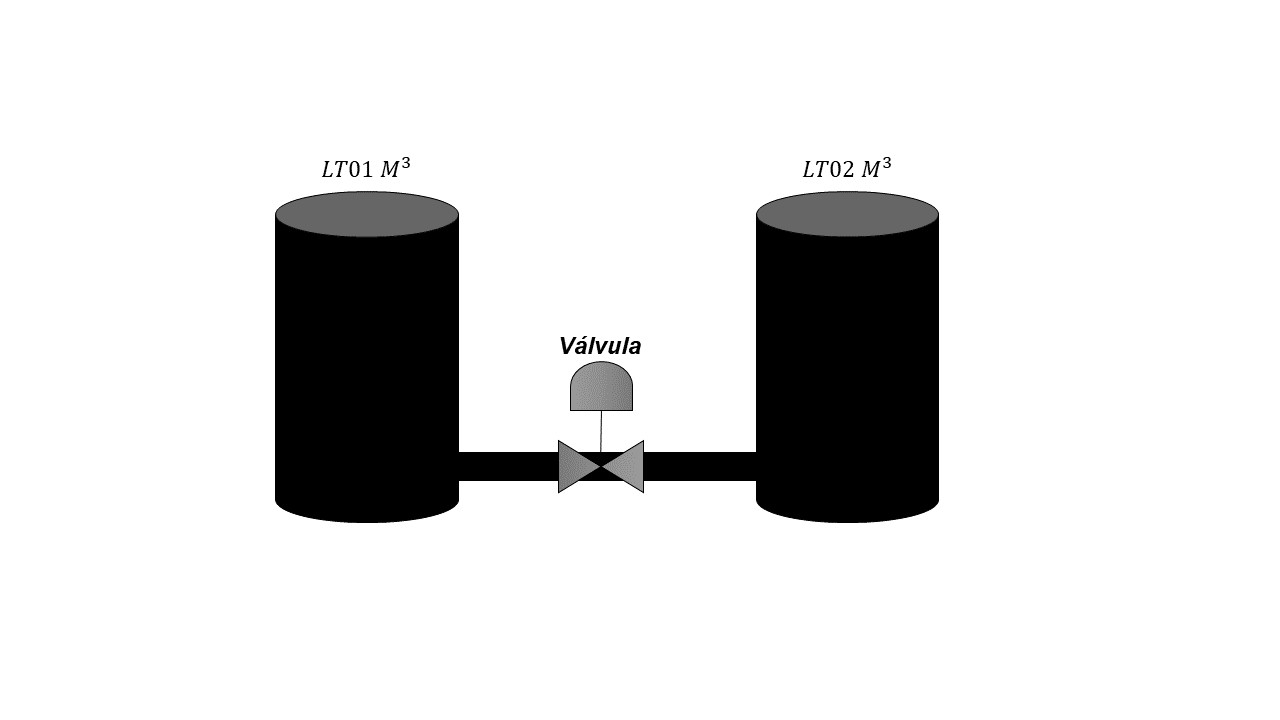
\includegraphics[width=1\linewidth]{Resultados/Figuras/esquema}
	Fonte: Elaboração própria 
\end{figure}

Na Figura \ref{fig:esquema} um esquema prático para evitar a escassez de água e o consumo em horários de pico. Este é um esquema muito simples de como a hora do dia pode ser melhorada para o armazenamento de água.

Na \ref{q3} o tanque tem como máximo nos dados $4,256 m^3$ de dano em litros $4256$L para atender esta demanda e manter o tanque quase cheio ou sempre cheio o fluxo de entrada tem que estar entre $[238,302] \ m^3/h$ fluxo de gravidade tem que estar entre $[126,182] \ m^3/h$ fluxo de retorno entre $[110,144] \ m^3/h$ pressão de sucção entre $[1.92,4.24] mca$, pressão de retorno entre $[21,24] \ mca$.

Para \ref{q4}, o ponto de equilíbrio para não iniciar as bombas seria o fluxo FT01 $211 m^3/h$ FT02 $114 m^3/h$ FT03 $100m^3/h$ e o nível do tanque a $3,545 m^3$.

Ao \ref{q5}\ref{q5:a} o tanque deve estar a um nível de $4,00 m^3$ para que não precise funcionar com bombas nas horas de pico. 

\subsubsection{M\'ultiplas entradas e sa\'ida \'unica (MISO)}

Nesta \ref{etp:2} os modelos que foram mais cobertos no decorrer da dissertação são os modelos ARIMA ou aqueles derivados deste modelo e os modelos regressivos fora do LR têm múltiplas entradas e uma saída da variável que se prevê a LT01, as outras variáveis servem como suporte para melhorar os modelos do tipo ARX ou modelos com variáveis exógenas. Os modelos ARIMA sem a variável exógena são apenas uma entrada semelhante com LR.

\subsubsection{Decomposi\c c\~ao STL}

 \citeonline{Theodosiou20111178} A decomposição sazonal e tendencial utilizando o procedimento de Loess (STL) é utilizada para a decomposição aditiva da série temporal global. O STL realiza a decomposição aditiva dos dados por meio de uma sequência de aplicações do Loess mais suave, que aplica regressões polinomiais ponderadas localmente em cada ponto do conjunto de dados, sendo as variáveis explicativas os valores mais próximos do ponto cuja resposta está sendo estimada. 
 
 \begin{figure}[H]
 	\centering
 	\caption{Decomposição STL aditiva dos dados coletados}
 	\label{fig:stl-aditiva}
 	\includegraphics[width=1\linewidth]{"Resultados/Figuras/STL aditiva"}
 	
 	Fonte: Elaboração própria a partir de dados da SANEPAR (2018 a 2020)
 \end{figure}
 
 
 \begin{figure}[H]
 	\centering
 	\caption{Decomposição STL multiplicativa dos dados coletados}
 	\label{fig:stl}
 	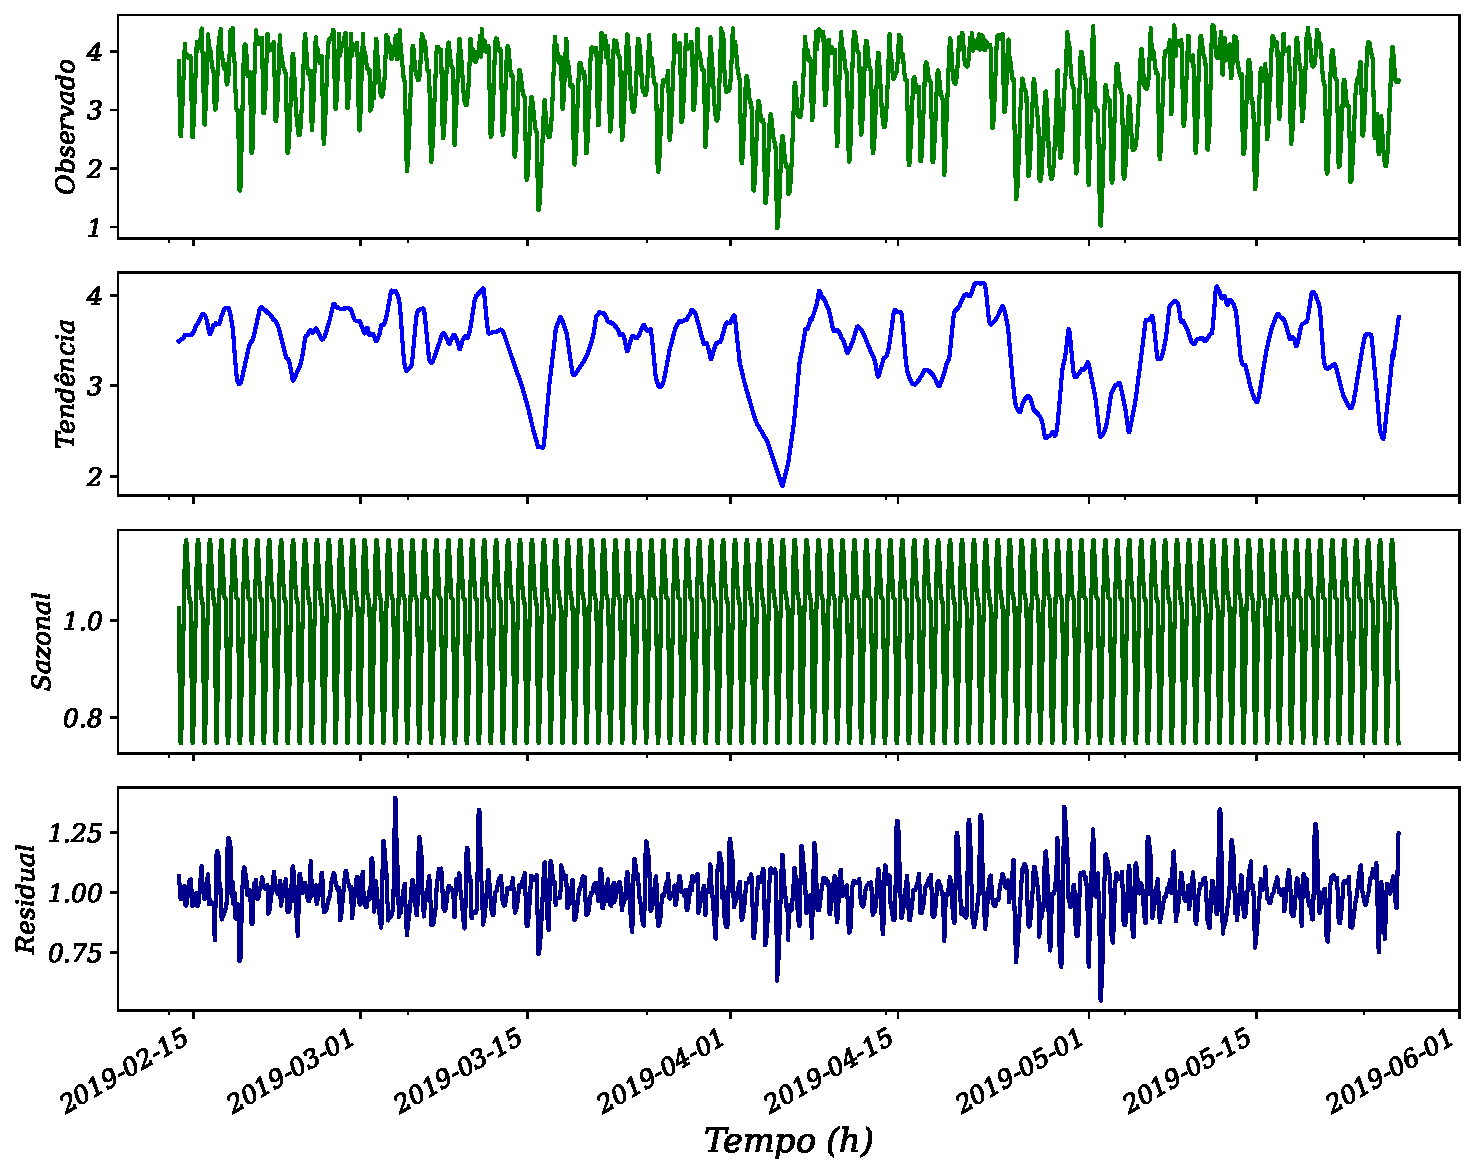
\includegraphics[width=1\linewidth]{Resultados/Figuras/STL}
 	
 	Fonte: Elaboração própria a partir de dados da SANEPAR (2018 a 2020)
 \end{figure}

Na \ref{q5}\ref{q5:b} resposta pode ser dada pelas Figuras \ref{fig:stl-aditiva} e \ref{fig:stl} como é observado tem tenacidade, sazonalidade e resido. 
 
Na decomposição, o objetivo é analisar se há tenacidade, sazonalidade e residência, olhando as Figuras \ref{fig:stl-aditiva} e \ref{fig:stl}, mostra que os dados têm ambas as análises. E com isso percebe-se que a série é estacionária, através do seguinte teste.

Teste de Dickey-Fuller (DF) Aumentado: 
\begin{itemize}
	\item Estatística de teste ADF     $-4.248$
\item $p-valor$                       $0.001$
\item atrasos utilizados         $21.000$
\item  observações              $1074.000$
\item valor crítico $(1\%)           -3.436$
\item valor crítico $(5\%)           -2.864$
\item valor crítico $(10\%)          -2.568$


Forte evidência contra a hipótese nula

Rejeitar a hipótese nula

Os dados não têm raiz unitária e estão estacionários em \ref{q5}\ref{q5:c}, pois a série está estacionária para identificar quais são as horas de pico entre 18h e 21h não é um trabalho fácil, como se você levasse a Figura \ref{fig:hist} para ver que no ano de 2020 houve um aumento na demanda naquelas horas.


\begin{figure}[H]
	\centering
	\caption{Violino no nível do reservatório}
	\label{fig:hist}
	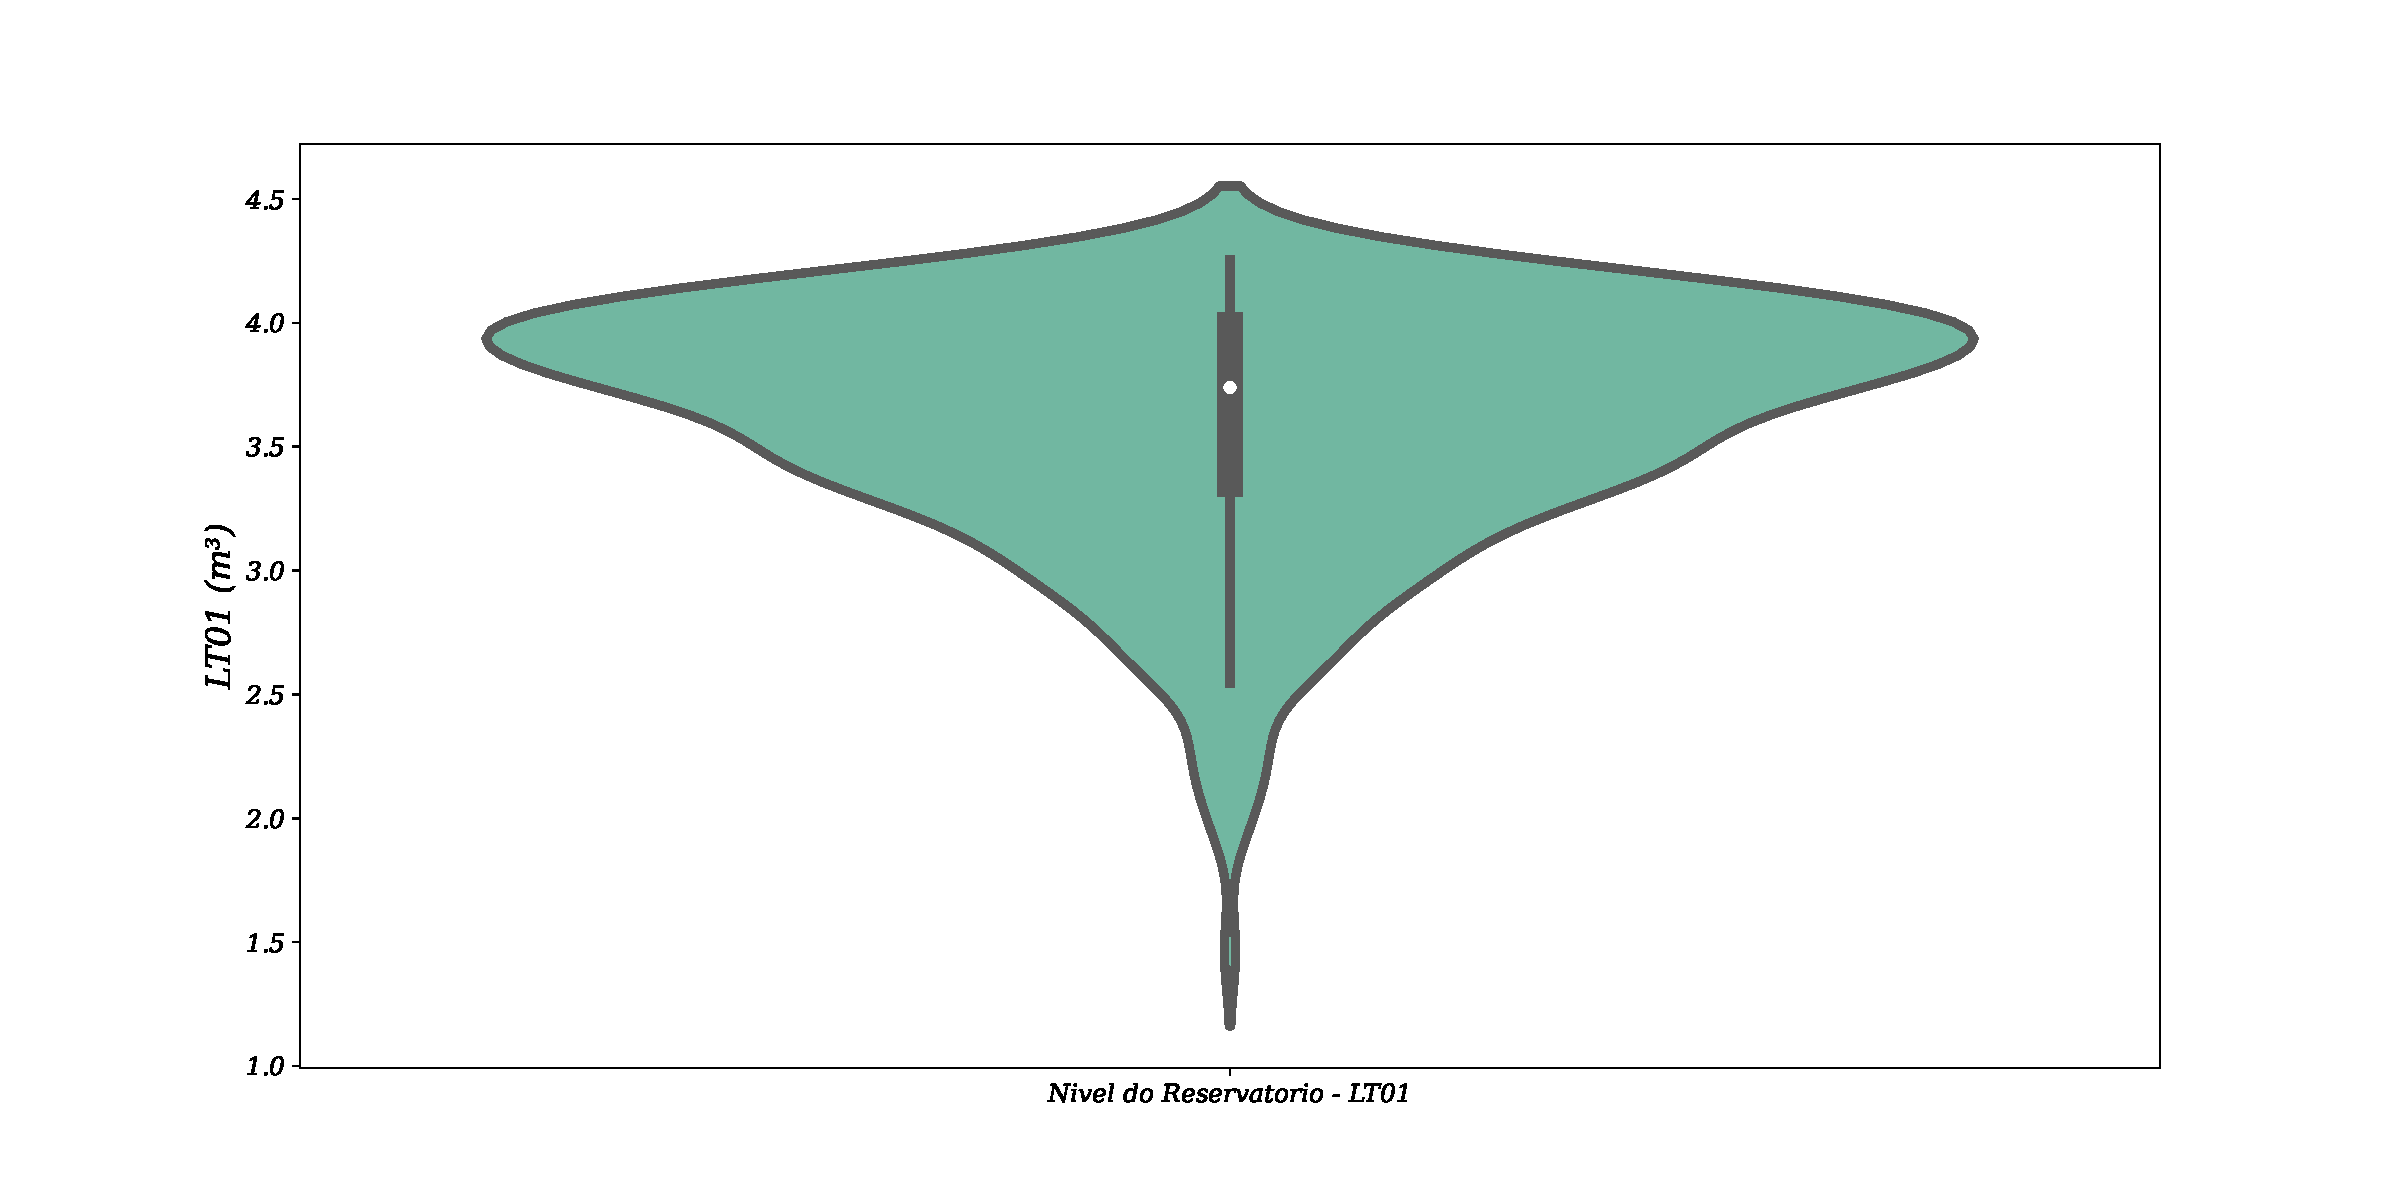
\includegraphics[width=1\linewidth]{Resultados/Figuras/viol}
	
	Fonte: Elaboração própria a partir de dados da SANEPAR (2018 a 2020)
\end{figure}

Assim, como dito na seção \ref{subsubsec:motivacao} as anomalias climáticas mais ocasionadas no ano 2020 e foi devido à falta de chuva naquele período.

Em \ref{q5}\ref{q5:d} nas horas de pico deve conter no tanque cerca de $[3.545,4.256] m^3$ para que não ligue as bombas.


\begin{figure}[H]
	\centering
	\caption{Violino da vazão de recalque}
	\label{fig:ft03}
	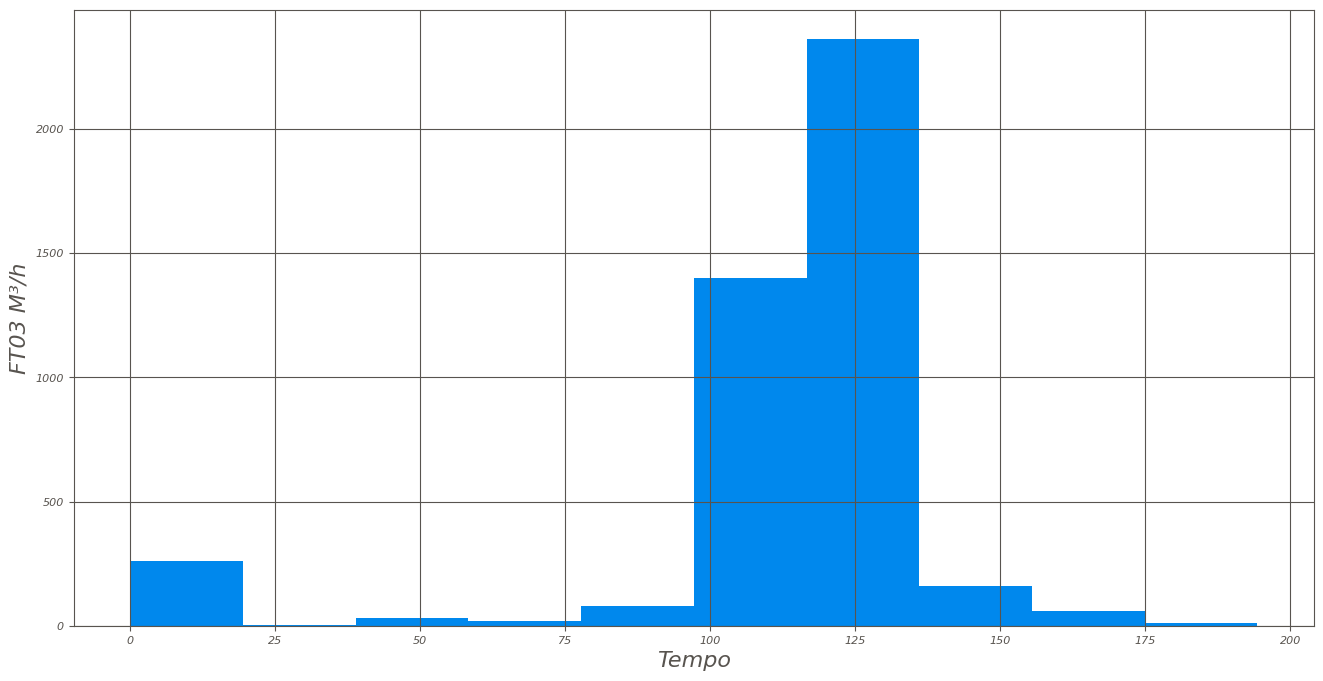
\includegraphics[width=1\linewidth]{Resultados/Figuras/ft03}
	
	Fonte: Elaboração própria a partir de dados da SANEPAR (2018 a 2020)
\end{figure}

Para \ref{q5}\ref{q5:e} é mostrado na Figura \ref{fig:ft03} como a vazão pode ser afetada com o nível do tanque. A vazão de recalque influencia mais o nível do tanque do que as outras vazões porque injeta água no tanque através da bomba que está mais próxima da base do tanque e as outras vazões por ter alguns valores ausentes não interferem tanto na amostra.


\end{itemize}

De acordo com o \citeonline{Reisen2017115}, o teste DF tem as seguintes equações

\begin{eqnarray}
	z_t&=& y_t+\theta \beta_t, \qquad t=1,\ldots, T, \label{eq:df3}\\	
\hat{\rho}_{\mathrm{DF}}-1&=&\frac{\sum_{t=1}^T z_{t-1} \Delta z_t}{\sum_{t=1}^T z_{t-1}^2} \label{eq:regdf}
\end{eqnarray}

De \eqref{eq:regdf} onde $\Delta z_t=z_t-z_{t-1}$. Sob a hipótese nula $\left(H_0\right)$ : `` $\rho=1$'', as estatísticas do teste DF e suas distribuições limitantes são dadas da seguinte forma:


\begin{eqnarray}
	T\left(\hat{\rho}_{\mathrm{DF}}-1\right)=T \frac{\sum_{t=1}^T z_{t-1} \Delta z_t}{\sum_{t=1}^T z_{t-1}^2}
\end{eqnarray}
e


\begin{eqnarray}
	\hat{\tau}_{\mathrm{DF}}&=&\frac{\hat{\rho}_{\mathrm{DF}}-1}{\hat{\sigma}_{\mathrm{DF}}\left(\sum_{t=1}^T z_{t-1}^2\right)^{-1 / 2}} \label{eq:df}
\end{eqnarray}

De \eqref{eq:df} onde $\hat{\sigma}_{\mathrm{DF}}^2=T^{-1} \sum_{t=1}^T\left(\Delta z_t-\left(\hat{\rho}_{\mathrm{DF}}-1\right) z_{t-1}\right)^2 .$



Suponha que $\left(z_t\right)_{1 \leq t \leq T}$ são dadas por \eqref{eq:df3}, então quando $\rho=1$,


\begin{eqnarray}
	T\left(\hat{\rho}_{\mathrm{DF}}-1\right) \stackrel{d}{\longrightarrow} \frac{W(1)^2-1}{2 \int_0^1 W(r)^2 \mathrm{~d} r}-\left(\frac{\theta}{\sigma}\right)^2 \frac{\pi}{\int_0^1 W(r)^2 \mathrm{~d} r}, \text { como } T \rightarrow \infty \\
	\hat{\tau}_{\mathrm{DF}} \stackrel{d}{\longrightarrow}\left[1+2(\theta / \sigma)^2 \pi\right]^{-1 / 2}\left\{\frac{W(1)^2-1}{2\left(\int_0^1 W(r)^2 \mathrm{~d} r\right)^{1 / 2}}-\frac{(\theta / \sigma)^2 \pi}{\left(\int_0^1 W(r)^2 \mathrm{~d} r\right)^{1 / 2}}\right\} \\
	\quad \operatorname{como} T \rightarrow \infty\label{eq:df2}
\end{eqnarray}


De \eqref{eq:df2} onde $\stackrel{d}{\longrightarrow}$ denota a convergência na distribuição e onde $\{W(r), r \in[0,1]\}$ denota o movimento browniano padrão.

Esse teste na literatura é chamado de teste ACF para testar se a série é o não estacionária, basicamente se a série tiver um valor de raiz unitária é uma série não estacionária, do contrario como acontece com os dados coletados se torna uma série estacionária.


\begin{figure}[H]
	\centering
		\caption{Autocorrelação e Autocorrelação parcial}
	\label{fig:acf}
	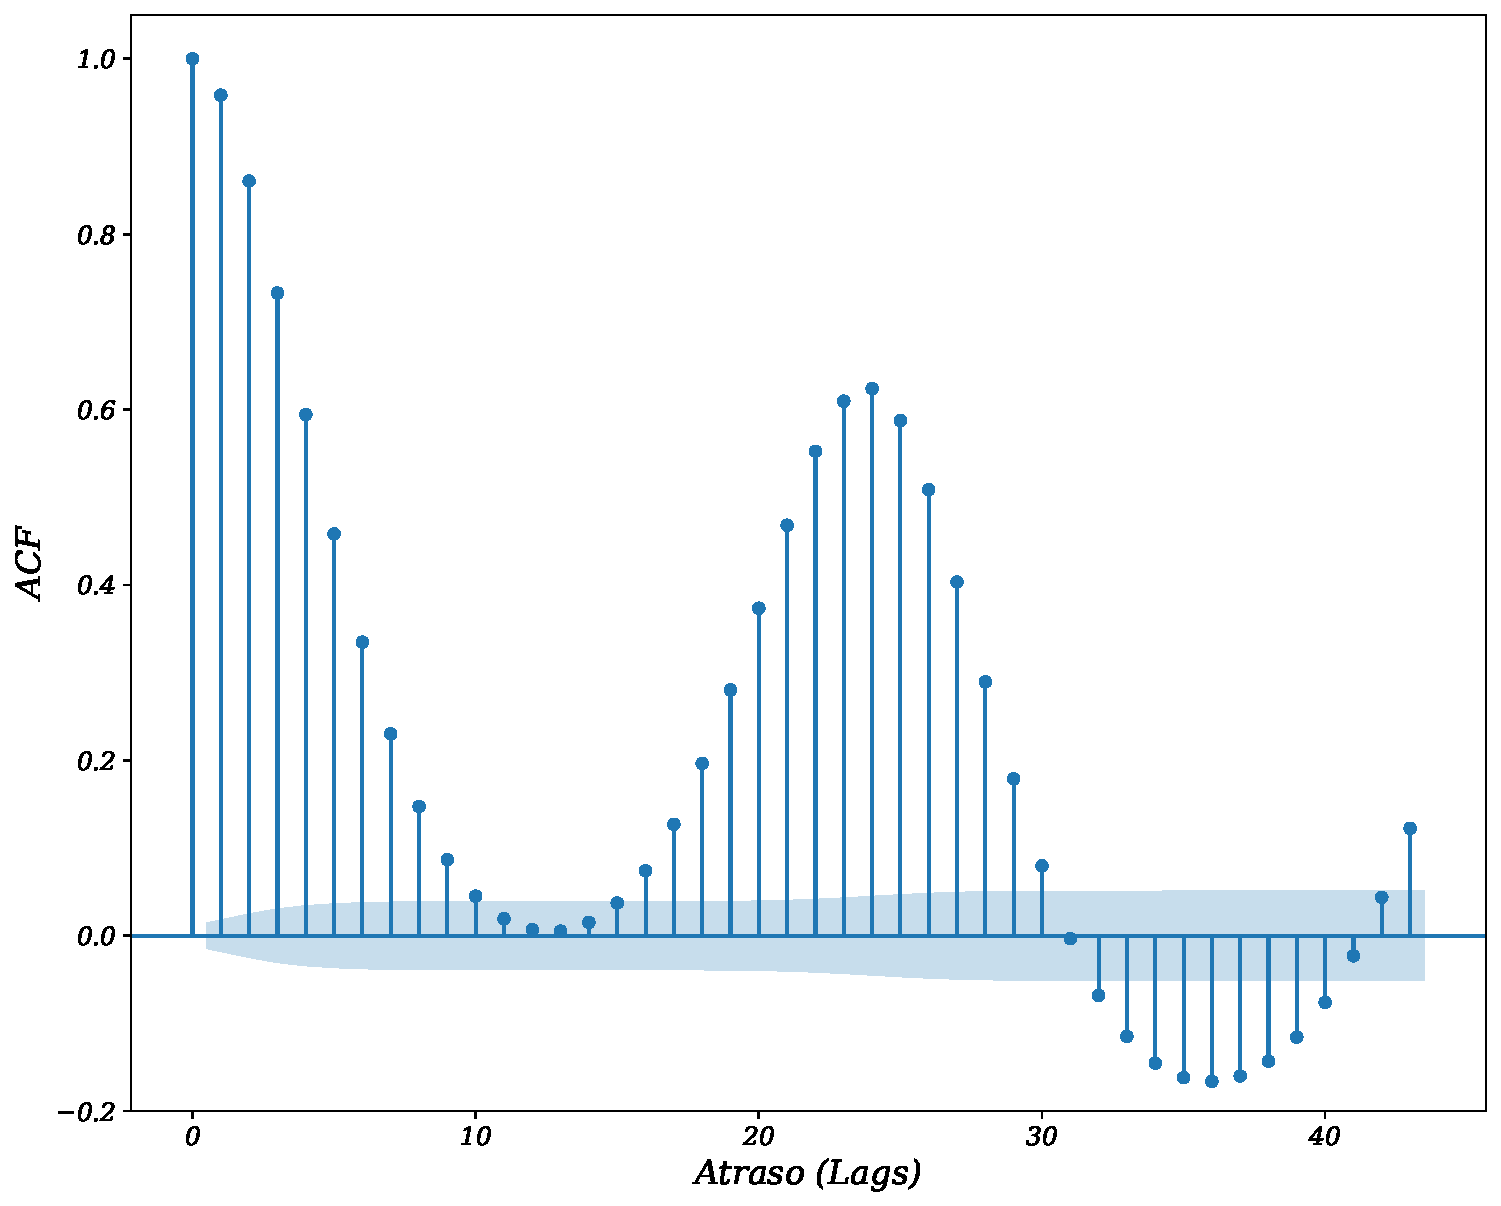
\includegraphics[width=1.1\linewidth]{Resultados/Figuras/acf} 
	
\end{figure}	
\begin{figure}[H]
	\centering
		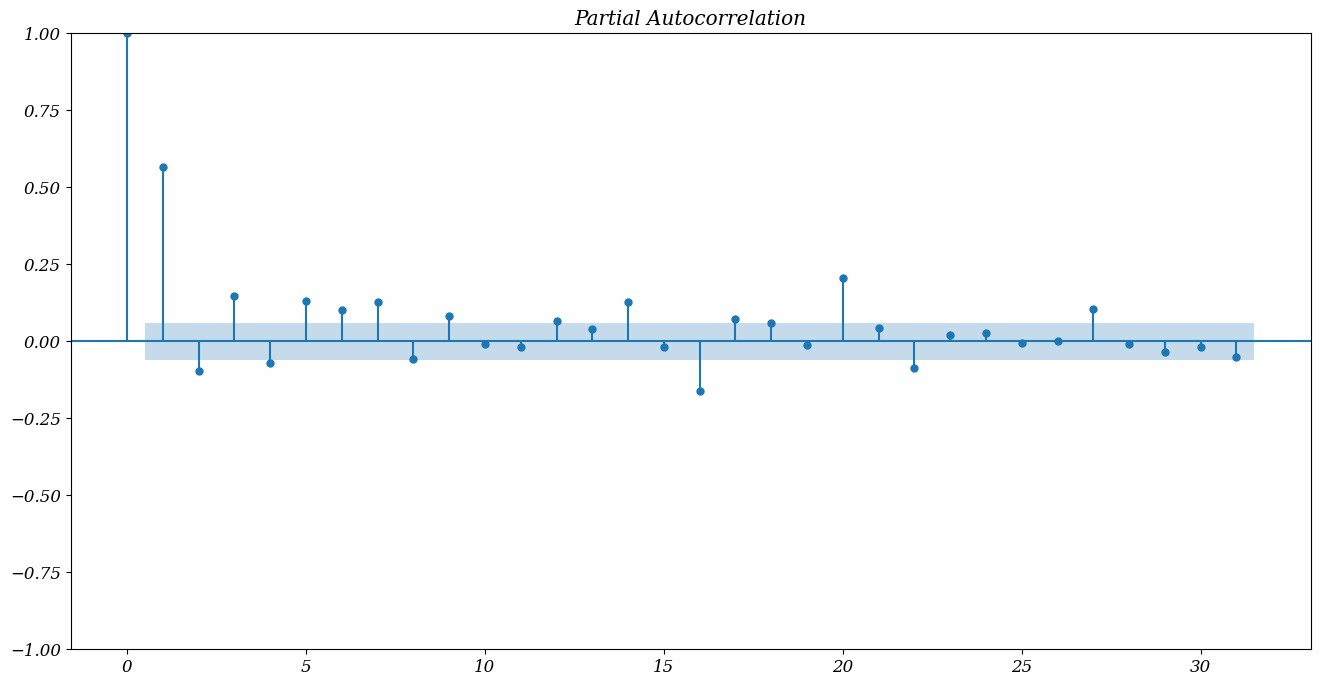
\includegraphics[width=1.1\linewidth]{Resultados/Figuras/pacf}

	Fonte: Elaboração própria a partir de dados da SANEPAR (2018 a 2020)
\end{figure}


Na Figura \ref{fig:acf} tem a diferença entre a autocorrelação e a autocorrelação parcial (PACF) é quase um detalhe em uma ACF temos a correlação direta e indireta e em uma PACF apenas a correlação direta. 

O intervalo de confiança por padrão é 95\%, mostrado como essa marca azul. Observações que estão para fora da marca são consideradas estatisticamente correlacionadas.

As correlação da Figura \ref{fig:acf} é a explicação do teste de DF, entendo isso pode ser visto o próximo passo que é  a análise do ruído branco em meados a gráfico, Uma série ruído branco é uma série na qual a média 0, a variância é constante ao longo da série toda e não há correlação entre os períodos de tempo. O valores de uma série ruídos brancos são totalmente aleatórios, ou seja, essa é um tipo de série que não é previsível.

\begin{figure}[H]
	\centering
	\caption{Ruído branco}
	\label{fig:ruido-branco}
	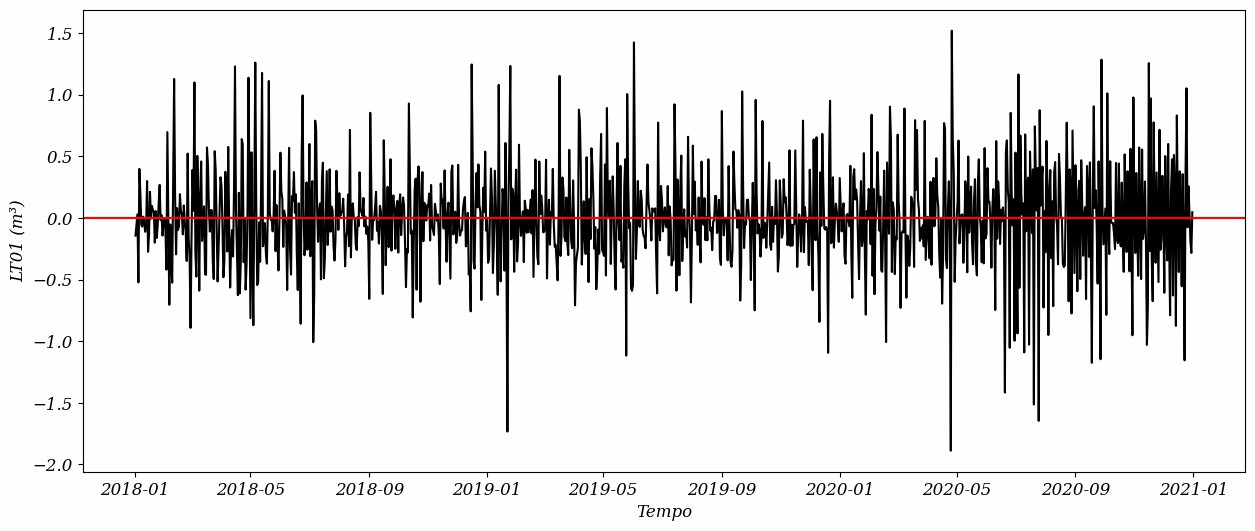
\includegraphics[width=1\linewidth]{Resultados/Figuras/ruido-branco}
	
	Fonte: Elaboração própria a partir de dados da SANEPAR (2018 a 2020)
\end{figure}

Da Figura \ref{fig:ruido-branco} uma série temporal pode ser ruído branco.
Uma série temporal é ruído branco se as variáveis são independentes e distribuídas de forma idêntica com uma média de zero.
Isso significa que todas as variáveis têm a mesma variância ($\sigma^2$) e cada valor tem uma correlação zero com todos os outros valores da série.
Mais para frente vamos mostrar o comprimento de zeros na variável prevista. Com isso encerra a \ref{etp:3}.

\subsubsection{Separa\c c\~ao dos Dados}

Na \ref{etp:4} tem um esquema de como foi dividido os dados em treino, teste e validação, essa pratica é comum para os profissionais de aprendizado de máquina, pois assim como não é passível processar os dados todos de uma vez, se você manosear dados em uma escala menor até pode ser realizado, mas tudo depende da máquina que esta sendo realizado o processamento dos dados, cada modelo em particular utiliza um certo acervo do seu computador para processar, se por exemplo você tiver trabalhando com um modelo de aprendizado profundo que é mais comum em processamento de imagem, a Nvidia tem sempre inovado com as suas GPUs e trazendo mais poder para processamento, com o recente lançamento da placa de vídeo $3090$ um sonho de consumo para games e os profissionais de aprendizado de maquina e profundo.

Em fim se o computador que foi realizado os processamento fosse um computador não tão bom, ainda poderia está sendo pensando que estaria em processamento, sem as inovação que foi estabelecida aos anos, o computador que foi realizado os cálculos dos modelos foi em partes um computador de processador $i5-3330$ e um notebook com $i7-5500$ ambos com 4 threads e o notebook com apenas 2 núcleos o $i5$ contem 4 núcleos. Cada um tem suas especificações de ser o melhor em algum certo ponto, mas sabendo que não é preciso de um de ultima geração para fazer tais processamento. E sim força de vontade para entende e aplicar em cada um.

A divisão mais básica que tem na literatura foi realizada aqui na separação dos dados, $70\%$ para treino e os $30\%$ restante para teste, dos $70\%$ tem mais uma divisão pegando $80\%$ dos $70\%$ para treino novamente e os $20\%$ para validação dos dados, tendo essa fórmula aplica na linguagem de programação para que não precisa ser contado todas as vezes que for mudado o modelo.

\subsubsection{Estrategia de Previs\~ao}\label{subsubsec:est}

Na \ref{etp:5} é abordado a forma que foi previsto os dados, em uma janela de horizonte de previsão bem maior do que o normal na literatura da estrategia de recursiva, sendo 1, 7, 14 e 30 dias previsto, essa estrategia para comparação dos modelos regressivo e modelos ARIMA, é bem vantajoso, pois cada modelo tem suas especificidade para prever em momentos com janela de tempo menor e com uma janela de muitos dias. Assim como explicado na seção \ref{subsubsec:modelos} se for previsão curta, alguns vai se sobre por em meio à outros modelos que foi feito aqui.

\subsubsection{Horizonte}

Na \ref{etp:6} é feito o horizonte de previsão, como dito na seção \ref{subsubsec:est} esse horizonte foi customizado baseado do método recursivo de prever as series temporais e a previsão do nível do tanque LT01. Os passos para prever a frente foi de 1, 7, 14 e 30 dias, já foi realizado uma estrategia com uma janela menor, mas para comparação dos modelos essa janela foi mais adequada.

\subsubsection{Modelos de previs\~ao e m\'etricas de desempenho}\label{subsubsec:modelos}

Da \ref{etp:7} as métricas utilizada aqui foi vista na seção \ref{subsec:metrica} foi utilizado aqui três das métricas mais usada na literaturar para previsão de tempo e comparação de modelos ARIMA e os modelos regressores.

    Em comparação com os modelos feito, pode ser visto que o modelo LR em um passo a frente tem tanto na modelagem de 24 horas quanto no pico de horas entre as 18 e 21 horas, foi o modelo que mais se saiu bem na previsão, logo em sequência os modelos MA, AR, SARIMA, ARIMA, SARIMAX, ARIMAX, ARX, LGBMRegressor, XGBRegressor e Random Forest Regressor, para curto prazo esses modelos estão em ordem de melhor para pior.
    
    Já em grande espaço de tempo como foi feito de 30 dias os modelos ARMA, AR, MA, ARIMA, ARIMAX, ARX, SARIMAX, SARIMA, XGBRegressor, Random Forest Regressor, LGBMRregressor e LR, seguindo a mesma lógica do melhor para o pior. Mas se olhar graficamente nos modelos que foi feito, os modelos com variáveis exógenas aparenta prever melhor do que os outros modelos, só analisando os dados nos apêndice tanto quando as Figuras de \ref{fig:1-AR-ARX-MA24} a \ref{fig:60-ARIMAX-SARIMA-SARIMAX24} quanto as Tabalas \ref{tb:1-24trn} a \ref{tb:60-24cm}   
    
    \subsubsection{Teste de Signific\^ancia}
    
    Na \ref{etp:9} os teste escolhido foi de \textit{Friedman e Nemenjy} no teste de Nemenyi, precisamos obter a diferença entre os rankings médios (linha média da tabela de classificação) entre todos os classificadores (comparando pares de classificadores). Se essa diferença for maior ou igual a um CD (distância crítica), podemos dizer que esses dois classificadores são significativamente diferentes um do outro. O CD é calculado como:
    
    \begin{eqnarray}
    	C D&=&q_\alpha \sqrt{\frac{k(k+1)}{6 N}}\label{eq:neme}
    \end{eqnarray}

De \eqref{eq:neme} o termo $q_\alpha$ é obtido de ($\alpha=0,05$):

\begin{table}[H]
	\centering
	\caption{Teste Nemenyi}
	\begin{tabular}{@{}clllllllll@{}}
		\toprule
		\multicolumn{1}{l}{\textbf{Nemenyi}} & \multicolumn{1}{c}{\textbf{0}} & \multicolumn{1}{c}{\textbf{1}} & \multicolumn{1}{c}{\textbf{2}} & \multicolumn{1}{c}{\textbf{3}} & \multicolumn{1}{c}{\textbf{4}} & \multicolumn{1}{c}{\textbf{5}} & \multicolumn{1}{c}{\textbf{6}} & \multicolumn{1}{c}{\textbf{7}} & \multicolumn{1}{c}{\textbf{8}} \\ \midrule
		\textbf{0}                           & 1,000                          & 0,001                          & 0,001                          & 0,001                          & 0,001                          & 0,001                          & 0,001                          & 0,001                          & 0,001                          \\
		\textbf{1}                           & 0,001                          & 1,000                          & 0,001                          & 0,001                          & 0,001                          & 0,001                          & 0,001                          & 0,001                          & 0,157                          \\
		\textbf{2}                           & 0,001                          & 0,001                          & 1,000                          & 0,847                          & 0,001                          & 0,001                          & 0,001                          & 0,001                          & 0,001                          \\
		\textbf{3}                           & 0,001                          & 0,001                          & 0,847                          & 1,000                          & 0,001                          & 0,001                          & 0,001                          & 0,001                          & 0,001                          \\
		\textbf{4}                           & 0,001                          & 0,001                          & 0,001                          & 0,001                          & 1,000                          & 0,001                          & 0,001                          & 0,001                          & 0,001                          \\
		\textbf{5}                           & 0,001                          & 0,001                          & 0,001                          & 0,001                          & 0,001                          & 1,000                          & 0,001                          & 0,001                          & 0,001                          \\
		\textbf{6}                           & 0,001                          & 0,001                          & 0,001                          & 0,001                          & 0,001                          & 0,001                          & 1,000                          & 0,001                          & 0,001                          \\
		\textbf{7}                           & 0,001                          & 0,001                          & 0,001                          & 0,001                          & 0,001                          & 0,001                          & 0,001                          & 1,000                          & 0,001                          \\
		\textbf{8}                           & 0,001                          & 0,157                          & 0,001                          & 0,001                          & 0,001                          & 0,001                          & 0,001                          & 0,001                          & 1,000                          \\ \bottomrule
	\end{tabular}

Fonte: Elaboração própria a partir de dados da SANEPAR (2018 a 2020)
\end{table}

O teste de Nemenyi (Nemenyi, 1963) é um teste \textit{post-hoc}, ou seja, é um teste de comparação múltipla que é usado após a aplicação de teste não paramétricos com três ou mais fatores.
    
Para calcular a estatística de teste $F_r$ de Friedman cria-se inicialmente uma tabela com os dados, colocando-se em cada linha uma amostra e cada coluna correspondendo a uma condição de teste. A seguir, as amostras ao longo das condições são ordenadas, da melhor situação para a pior. Se não houver empates, usa-se a equação \eqref{eq:fr} para determinar a estatística de teste $F_r$:

\begin{eqnarray}
	F_r&=&\left[\frac{12}{n k(k+1)} \sum_{i=1}^k R_i{ }^2\right]-3 n(k+1)\label{eq:fr}
\end{eqnarray}
  
  Na equação \eqref{eq:fr} $n$ é o número de linhas (ou amostras), $k$ é o número de colunas (ou condições) e $R_i$ é a soma dos postos da coluna (ou condição) $i$.   
 Seguindo a equação \eqref{eq:fr} têm o seguinte resultado nos dados da pesquisa.
 
 $statistic=8015.611,\ \ pvalue=0.0$ com o números de 26306 linhas x 9 colunas.
 
 \subsubsection{Compara\c c\~ao dos modelos}
 Nos modelos coletados com várias métodos de prever, com isso para ver melhor como cada modelo se comporta foi realizado a comparação dos modelos em base com o gráfico violino, assim observa quais os melhores entre os modelos coltado.
 
 \begin{figure}[H]
 	\centering
 	\caption{Comparação de modelos ARIMAS}
 	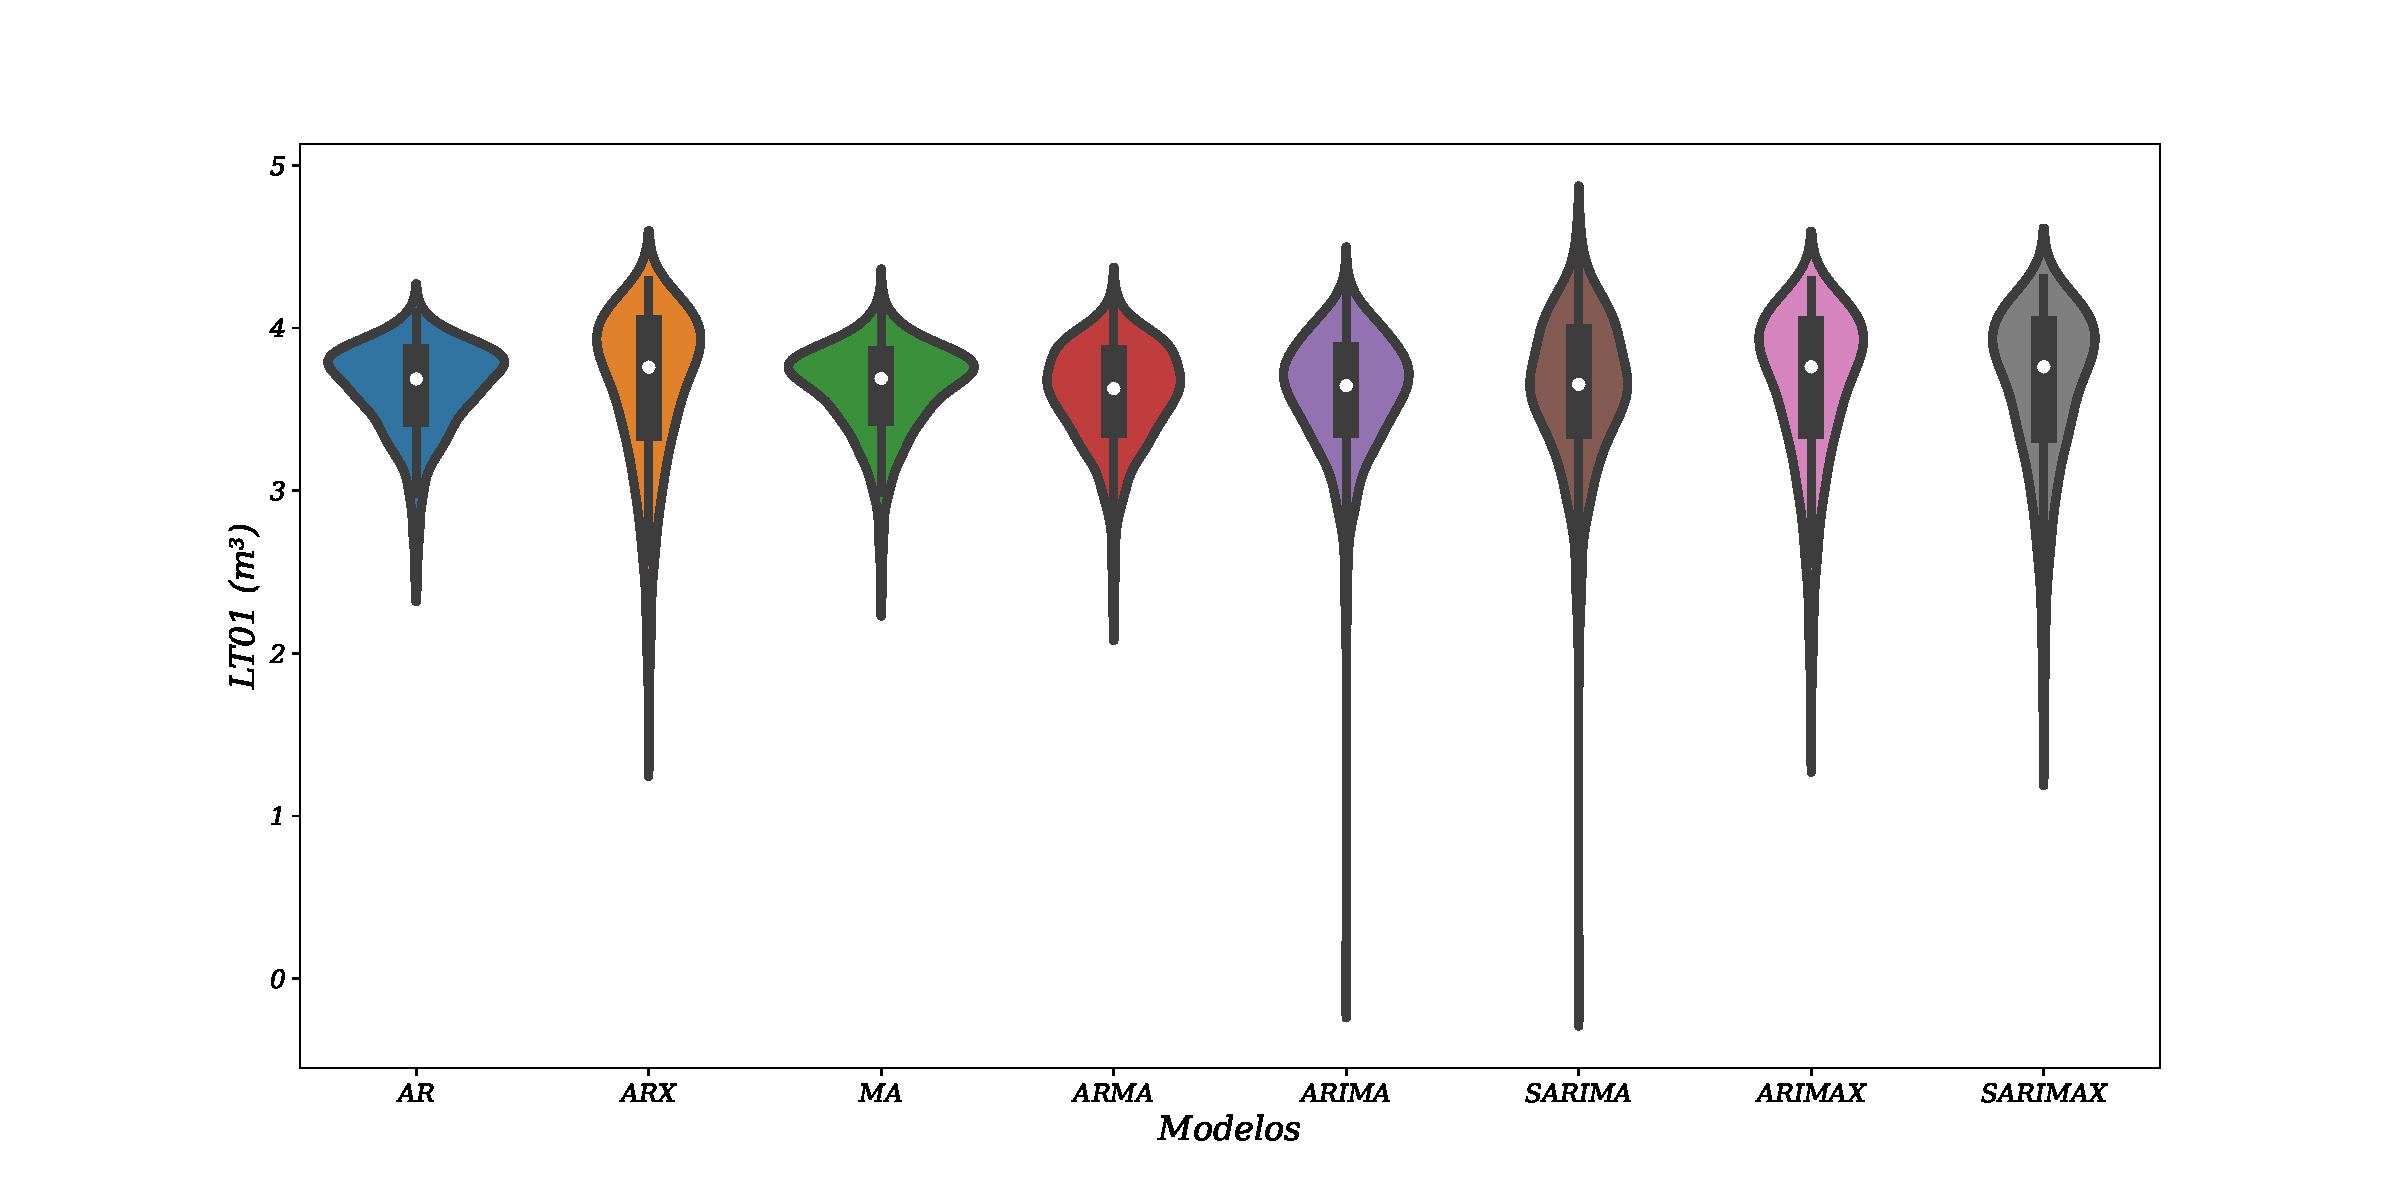
\includegraphics[width=0.9\linewidth]{Resultados/Figuras/modelos-arima}
 	
 	\label{fig:modelos-arima}
 	
 	Fonte: Elaboração própria a partir de dados da SANEPAR (2018 a 2020)
 \end{figure}
 
 
 \begin{figure}[H]
 	\centering
 	\caption{Comparação de modelos de regressão }
 	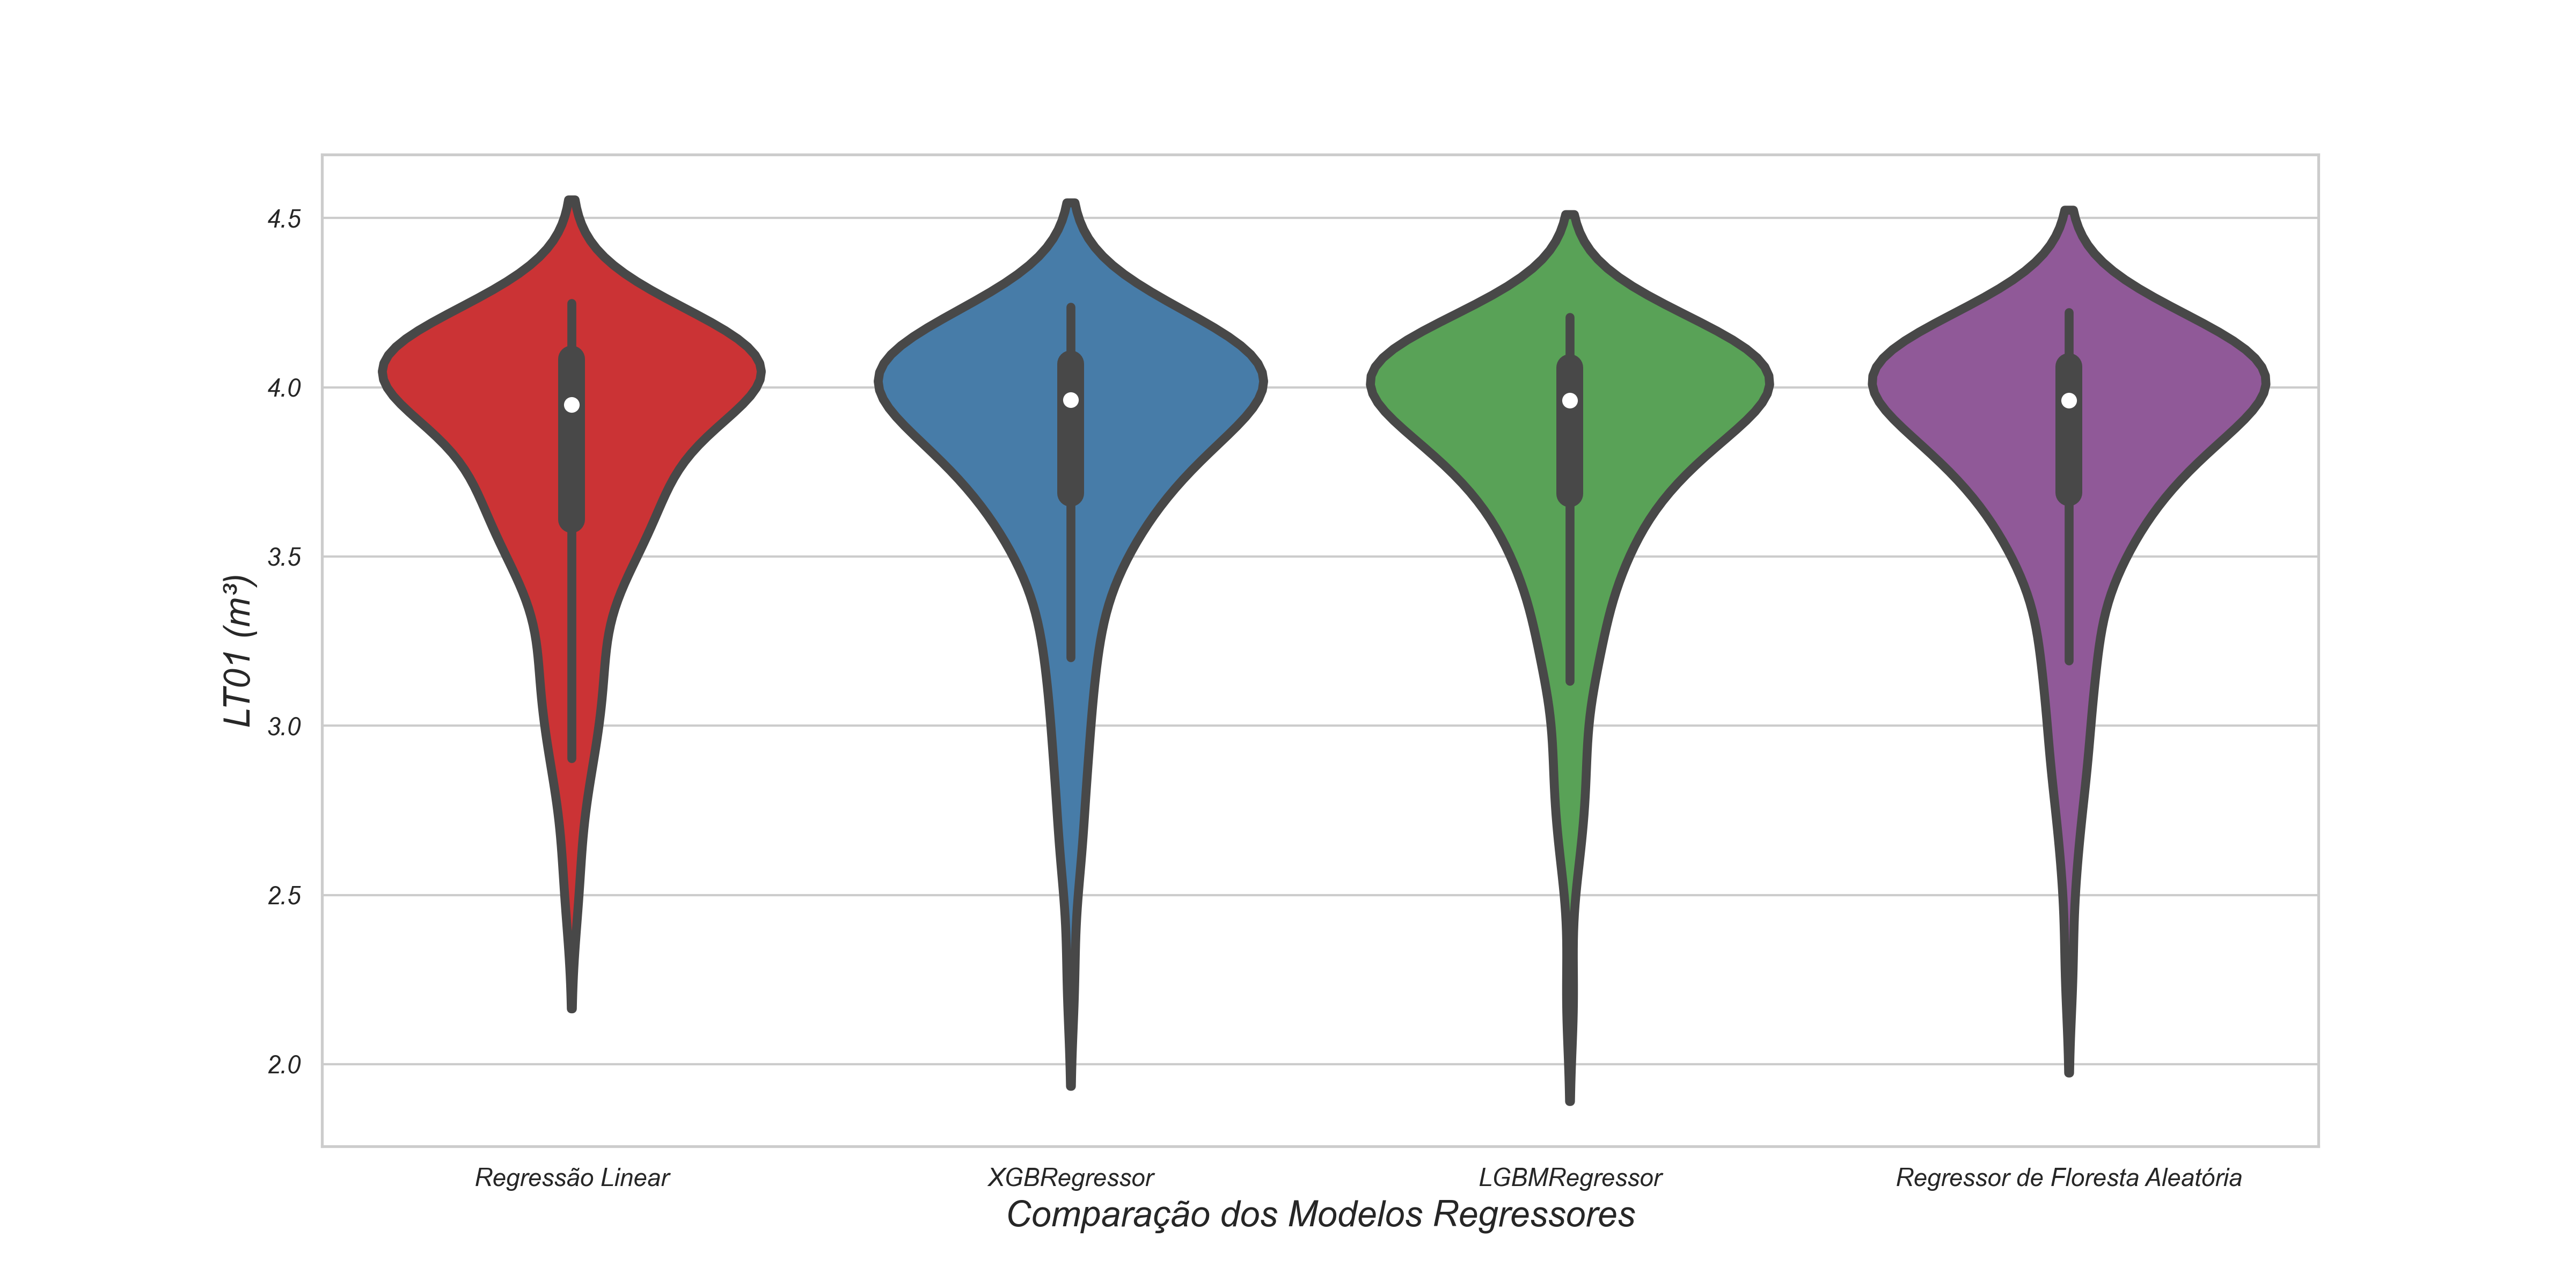
\includegraphics[width=0.9\linewidth]{Resultados/Figuras/violin-LR-XGB-LGBM-RF}
 	
 	\label{fig:violin-lr-xgb-lgbm-rf}
 	
 	Fonte: Elaboração própria a partir de dados da SANEPAR (2018 a 2020)
 \end{figure}


Em comparação com os modelos apresentado nas Figuras \ref{fig:modelos-arima} e \ref{fig:violin-lr-xgb-lgbm-rf} os modelos que pode ser observado que são os melhores levando em conta a modelagem dos dados, nos modelos ARIMA os melhores são AR, ARX, MA, ARMA, ARIMAX e SARIMAX, devido ao \textit{outliers} e ao limite inferior de alguns modelos, olhando para os modelos de gradiente e regressão, pode se notar que eles ficaram similar, devido a técnicas de otimização matemática Grid Search (do inglês pesquisa grande) e Randomized Search (do inglês pesquisa aleatória), que possibilitou a melhora do método utilizado. Em um horizonte de previsão pequeno o LR prevê melhor que os outros modelos, mas em um horizonte de previsão maior os modelos XGBoost e Light GBM estão prevendo com melhor rigor. O floresta aleatória está prevê com rigor também só vindo atrás do XGBoost em previsão de longo prazo.

O método de Ljung box é um método que pode ser estimados a longo prazo os modelos ARIMAS se a longo prazo eles ainda vão prever com eficiência nos dados, a longo prazo os modelos que melhor prevê são os modelos ARX, ARIMAX e SARIMAX com as variáveis exógena para modelos não linear ele consegue se manter por mais tempo prevendo do que os outros modelos ARIMA.  
 
  
    

    
